\documentclass[a4paper,10pt]{article}
\usepackage[utf8]{inputenc}
\usepackage{geometry} %自定义布局
\usepackage{multicol} %双栏
\usepackage{graphicx} %图像
\usepackage{amsmath} % 数学单位等等
\usepackage[runin]{abstract} %摘要修改 摘要标题添加到摘要正文段前
\usepackage{booktabs}%三线格
\usepackage{float}%浮点
\usepackage{cite}%引用
\usepackage{pdfpages}%pdf合并
\usepackage{caption}
\usepackage{graphicx, subfig}
\usepackage[colorlinks,
            linkcolor=blue,       %%修改此处为你想要的颜色
            anchorcolor=blue,  %%修改此处为你想要的颜色
            citecolor=blue,        %%修改此处为你想要的颜色,例如修改blue为red
            ]{hyperref}
\usepackage{appendix}
\geometry{a4paper,left=1.6cm,right=1.6cm,top=2cm,bottom=2cm}
\graphicspath{{picture/},{pics/}}
%opening
\title{Purification and Identification of Three Unknown Proteins}
%%%标题加粗
\author{}
\date{}


\begin{document}


\maketitle


\setlength{\absleftindent}{0pt}
\setlength{\absrightindent}{0pt}
\setlength{\abstitleskip}{-1.5em}
\abslabeldelim{:}
\renewcommand{\abstractnamefont}{\itshape\bfseries}
\renewcommand{\absnamepos}{flushleft}


\begin{abstract}
\textit{\small Protein purification is a critical topic in molecular biology. Chromatography is frequently employed in the separation and purification processes of biochemical molecules. The purified proteins can be further analyzed using techniques such as SDS-PAGE and western blot. In this experiment, samples of three unknown proteins were isolated and identified, and their yields were calculated. Initial purification was conducted using ion exchange chromatography (IEX) and gel filtration chromatography (GFC), followed by protein concentration determination using the Bradford method, and subsequent SDS-PAGE/WB and bioinformatics analysis for protein characterization. The results showed successful separation and identification of the three proteins as Cytochrome C, Myoglobin, and Ferritin, with concentrations of 1.7 mg/mL, 2.0 mg/mL, and 1.9 mg/mL, respectively. However, inconsistencies observed in SDS-PAGE/WB results may indicate the need for further improvements in the experimental procedures to avoid biased yield values. }
\end{abstract}


\hrule


\begin{multicols}{2}
\section{Introduction}


%\noindent %无缩进
Protein separation and purification are essential techniques in the field of biochemistry, allowing for the isolation and purification of one or more proteins from complex mixtures \cite{liu2020recent}. Chromatography is a commonly used protein separation technique in academia. Protein mixtures are passed through a column filled with a stationary phase, allowing proteins with different characteristics to be separated based on properties such as hydrophobicity, size, charge, and biorecognition. Ion exchange chromatography (IEX) utilizes a stationary phase with charged functional groups to separate proteins based on their charge properties \cite{rajesh2018cellulose}. Gel filtration (GF), also known as size exclusion chromatography, separates proteins based on their molecular weight \cite{cai2017top}. The purity of separated proteins can be determined by using techniques such as SDS-PAGE and western blot (WB). In SDS-PAGE, proteins with smaller sizes and negative charges move faster during electrophoresis, leading to the separation of proteins with different weights \cite{katorcha2018analysis}. WB allows for the detection and quantification of specific proteins within a complex mixture. After separation using SDS-PAGE, the gel is transferred to a container, and the target protein is identified and detected using specific antibodies \cite{desire2023development}. In this experiment, a combination of IEX and GF will be used to separate a mixture of three unknown proteins. Protein concentrations will be determined using the Bradford method, and bioinformatics analysis will be used in conjunction with the results of SDS-PAGE and western blot to identify the protein components in the mixture.

\section{Material and Method}



\begin{center}
%{\footnotesize Table 1. Materials needed for this experiment}
{Table 1. Materials needed for this experiment}
\begin{table}[H]
%\footnotesize
\begin{tabular}{ll}
\toprule [1pt]
\textbf{Equilibration Buffer}&\textbf{Explanation  }\\
\hline
Tris-HCL&100mM\\
\hline
\textbf{Elution Buffer}&\\
\hline
NaCl&2M\\
Tris-HCl&100mM\\
\hline
\textbf{GFC Buffer}&\\
\hline
Tris-HCl&50mM\\
\hline
\textbf{SDS sample Buffer}&\\
\hline
Tris-HCl&62.5mM\\
SDS&2\%(w/v)\\
Glycerol&10\%(v/v)\\
Bromophenol blue&0.25\%(w/v)\\
$\beta$-mercaptoethanol&5\%(v/v)\\
\hline
\textbf{Running Buffer}&\\
\hline
Tris&0.025M\\
Glycine&0.192M\\
SDS&10\%\\
\hline
\textbf{12\% Seperating Gel}&\\
Acrylamide solution&2.7mL\\
dd water&5.02mL\\
Tris-HCl&1.13mL\\
SDS&0.09mL\\
Ammonium persulphate&0.05mL\\
TEMED&0.01mL\\
\hline
\textbf{5\% Stacking Gel}&\\
Acrylamide solution&0.375mL\\
dd water&1.93mL\\
Tris-HCl&0.75mL\\
SDS&0.03mL\\
Ammonium&15\textmu L\\
TEMED&6\textmu L\\
\bottomrule [1.5pt]
\end{tabular}
\end{table}
\end{center}


\subsection{ Ion exchange chromatography (IEX)}
Equilibrate the column containing diethyl amino ethyl (DEAE)-Trisacryl by pre-equilibration buffers. Then, pump 4 mL of the original sample into the column. Collect 2 mL of unbound proteins (most concentrated) in a labeled centrifuge tube and place it on ice. After all unbound samples have passed through the column, pump elution buffer to elute the remaining bound proteins. Collect the most concentrated 2 mL sample and store the collected samples at -20\textcelsius\ for further use.


\subsection{Gel filtration chromatography (GFC)}
The column containing Sephacryl S200HR was pre-equilibrated in GFC buffer. Then, 0.5 mL of the bound protein was pumped in using a syringe. Starting from when the color reached the bottom of the column, elution buffer was collected in 25 fractions of 0.5 mL each, labeled in order,  stored at -20\textcelsius.


\subsection{Scanning spectrophotometry}

The wavelength with the maximum absorption peak was determined by scanning the original samples between 350-650 nm. The equipment was zeroed using the GFC buffer, and the absorbance (ABS) of 25 fractions was measured. Spectrophotometry measurement data were then generated.


\subsection{Bradford assay}
Dilute 1.0 mg/mL IgG using equilibration buffer, add 20 \textmu L of IgG to 1 mL of Bradford dye reagent, and mix for 5 minutes. Generate a standard curve between 0 and 1 mg/mL by measuring absorbance at 595 nm. Protein samples were diluted fivefold to ensure absorbance fell within the calibration curve, and 20 \textmu L of each sample was mixed with 1.0 mL of Bradford dye reagent and incubated for 5 min at room temperature. Blue absorbance was measured at 595 nm using different blanks. Calculate the sample protein concentration from the calibration curve.


\subsection{SDS-PAGE}
Prepare 12\% separating gel and 5\% stacking gel in advance. Dilute the protein samples (original sample, two fractions from IEX, two peak fractions from GFC) to 0.25 mg/mL, then add each sample to two positive controls, 20 \textmu L 5x -SDS Loading Buffer, and 80 \textmu L protein Mix and heat at 95°C for 5 minutes. These prepared samples will be used for SDS-PAGE and WB . After heating, add 20 \textmu L of sample and 10 \textmu L of marker to each well . After adding running buffer, samples were electrophoresed at 80V for 30 minutes and then at 120V for approximately 1 hour until the dye reached the edge of the gel. After electrophoresis, the gel was stained with Coomassie blue in a beaker for 1 hour and rinsed repeatedly during destaining. Finally, capture the gel.


\subsection{Western blottings}
Place the unstained gel after SDS-PAGE into a WB transfer device. Proteins were transferred to nitrocellulose membrane at 100V for 1 h. Membranes were blocked with 5\% milk and incubated with primary antibodies for 1 h. After washing with 0.1\% TBS-T, incubate with secondary antibody for half an hour. After adding enhanced chemiluminescence, the signal intensity was photographed and recorded.


\subsection{Bioinformatic analysis }
The partial sequence of the protein is used to query the protein name through BLASTP. Further analysis was performed using Expasy to determine their MW and pI values. Data analysis was performed using ImageJ to measure distances in SDS-PAGE gel photographs and grayscale values in WB.


\iffalse
\begin{center}
{\footnotesize Table 2. Outline of the mutagenesis for each plate}
\vspace{0pt}
\begin{table}[H]
\footnotesize
\begin{tabular}{ccccc}
\toprule [1.5pt]
Plate Number&Cell dilution to be plated&Plate type&Tryptophan concentration(\textmu g/mL)&Treatment\\
\hline
1&$10^0$&SA3&0&$Trp^+$ strain and $Trp^-$ strain\\
2&$10^0$&SA3&0&None\\
3&$10^0$&SA2&1&None\\
4&$10^0$&SA1&0.25&None\\
5&$10^{-5}$&NA&Non-limiting&None\\
6&$10^{-6}$&NA&Non-limiting&None\\
7&$10^0$&SA2&1&Spot test with 1\% MMS\\
8&$10^0$&SA2&1&Spot test with 1\% MMS\\
9&$10^0$&SA2&1&Spot test control (water)\\
10&$10^0$&SA1&0.25&Treat with 1\% MMS then plate\\
11&$10^0$&SA2&1&Irradiate with UV light for 20 sec\\
12&$10^0$&SA2&1&Irradiate with UV light for 40 sec\\
\bottomrule [1.5pt]
\end{tabular}
\end{table}
\end{center}
\fi


%\begin{figure}[htbp]
%\centering
%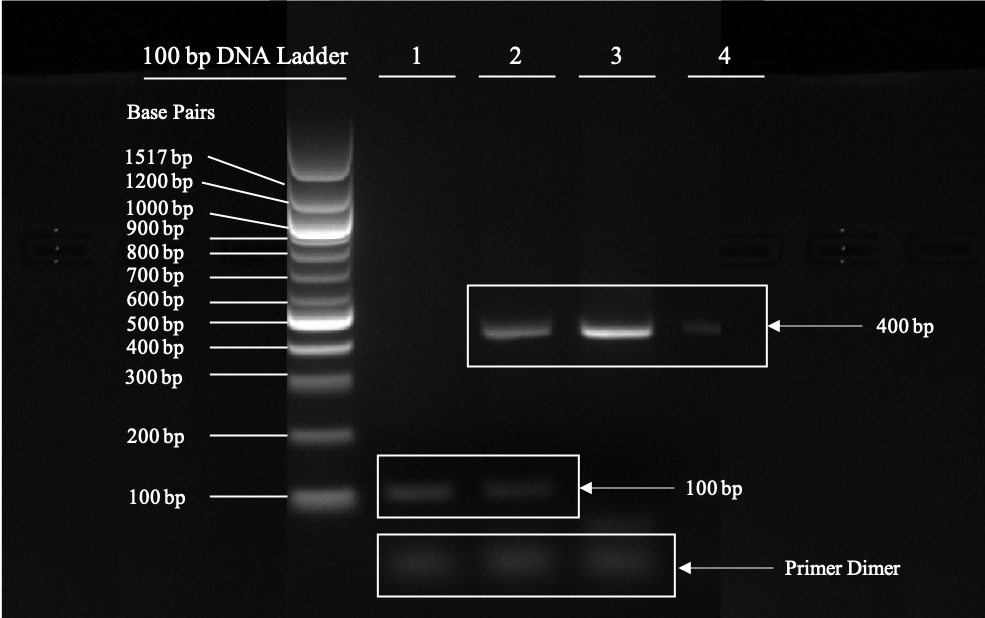
\includegraphics{tpa25.png}
%\caption{bionux}
%\end{figure}


\section{Results and Analysis}


\subsection{pI and WM analysis}
The results of electrophoretic analysis including isoelectric focusing and native PAGE are shown in Figure 1. Three unknown proteins were separated in both methods, indicating that protein mixtures can be separated based on pI and MW. The pI and MW for each band can be derived. The order of a, b, c does not necessarily correspond to the order of 1, 2, 3. Prior to GFC, the remaining two proteins can be separated regardless of the order of protein separation. In summary, IEX was confirmed to be suitable for separating three target proteins, and GFC was confirmed to be suitable for purifying three target proteins.


\begin{figure}[H]
\centering
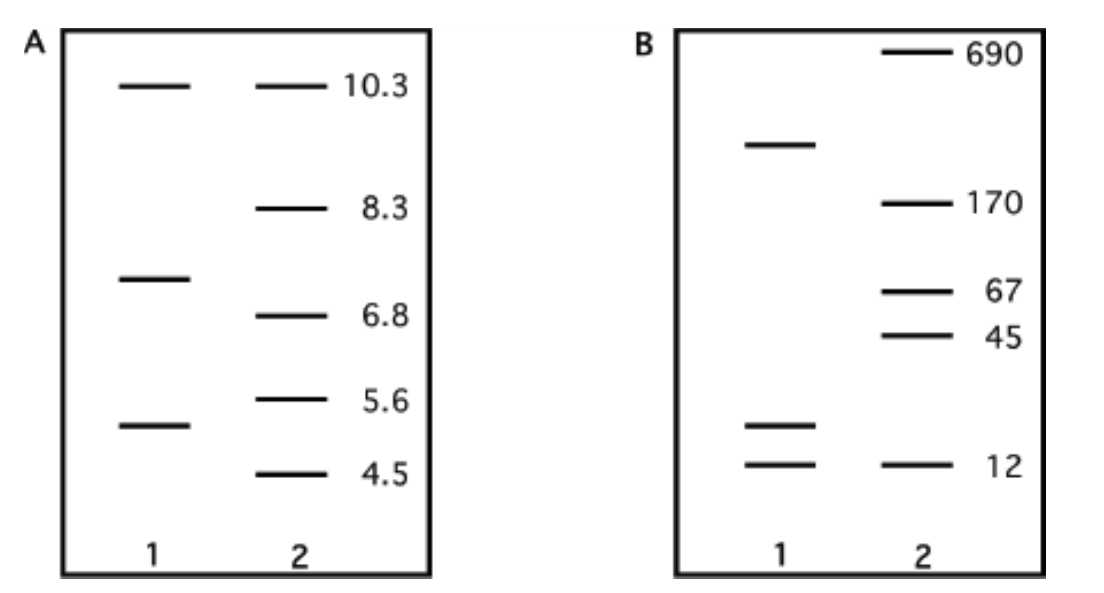
\includegraphics[width=0.45\textwidth]{sds.png}
\captionsetup{font={scriptsize,bf,stretch=1}}
\caption{\scriptsize \textbf{Electrophoretic Analyses Results of Protein Mixture. The picture on the left is isoelectric focusing of a protein sample. The three protein bands are represented by 1, 2, and 3. The picture on the right is the polyacrylamide gel electrophoresis result of the protein sample. The three protein bands are represented by a, b, and c. }}
\label{fig1}
\end{figure}


\begin{center}
{Table 2. Count of bacterial colonies on each plate}
\vspace{0pt}
\begin{table}[H]
\setlength{\tabcolsep}{5pt}

\begin{tabular}{llll}
\toprule [1pt]
Component&pI value & Component & MW\\
\hline
protein 1 & 10.3 & protein a & 298\\
protein 2 & 7.5 & protein b & 19\\
protein 3 & 5.3 & protein c & 12\\
\bottomrule [1pt]
\end{tabular}
\end{table}
\end{center}


\subsection{Anion Exchange Chromatography}
The two separated samples were pink and brown (Fig. 2). Pink protein a will be separated because it has a pI of 10.3, is positively charged within the column, and can pass directly through the column. The other two brown proteins, both with pI values below 9.0, are negatively charged and therefore bind to the column and cannot be separated from each other during elution.


\begin{figure}[H]
\centering
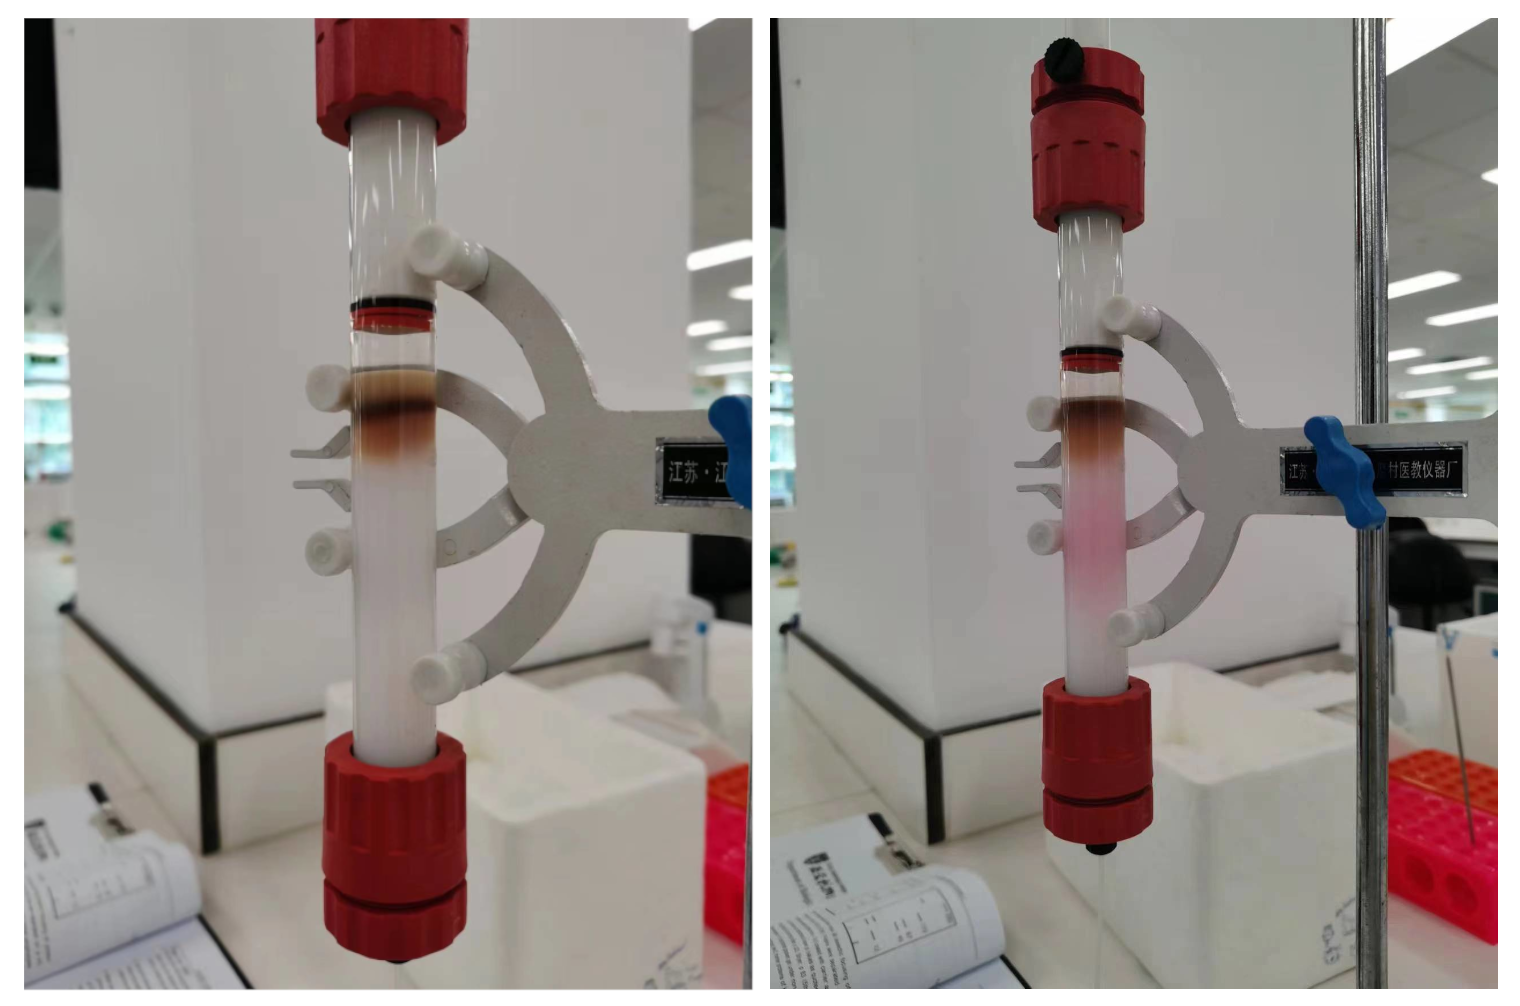
\includegraphics[width=0.45\textwidth]{iex.png}
\captionsetup{font={scriptsize,bf,stretch=1}}
\caption{\scriptsize \textbf{Ion exchange chromatography images, the left image is an image of uneluted brown protein(bound protein), and the right image is an image of eluting pink protein(unbound protein).}}
\label{fig2}
\end{figure}


\subsection{Gel Filtration Chromatography}
Brown proteins were further separated using differences in molecular weight. Since the mass difference between proteins b and c is greater than 10\%. Larger proteins penetrate porous gels more easily and remain inside the gel longer, while smaller proteins move quickly through the gel channels, so both proteins are expected to be separated. The results of 25 tubes containing two protein peaks are shown in Figure 3. Color depth is positively correlated with protein concentration. And the discontinuous appearance of two color depths tubes means the separation is successful.


\iffalse
\begin{figure*}
\centering
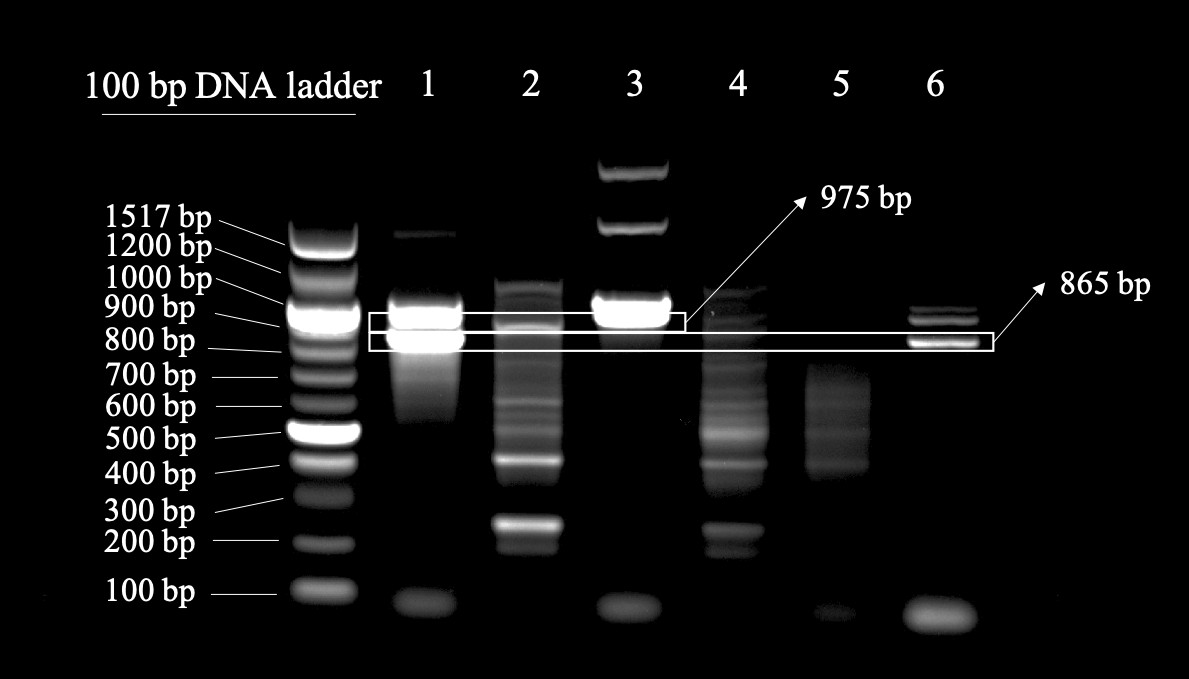
\includegraphics[width=0.95\textwidth]{gel.jpg}
\captionsetup{font={scriptsize,bf,stretch=1}}
\caption{\scriptsize \textbf{PCR verification for putative transformants 1 and 2. Lanes 1 and 2 were set as negative controls which added the genome of the negative strain as a template. Lanes 3 and 4 added the genome of transformant 1 as a template. Lanes 5 and 6 added the genome of transformant 2 as a template. Samples of lanes 1, 3 and 5 were amplified DNA with diagnostic primers ANID\_08549F and ANID\_08549R. Samples of lanes 2, 4 and 6 were amplified DNA with diagnostic primers ANID\_08549F and Af-Revers.}}
\label{fig3}
\end{figure*}
\fi


\begin{figure}[H]
\centering
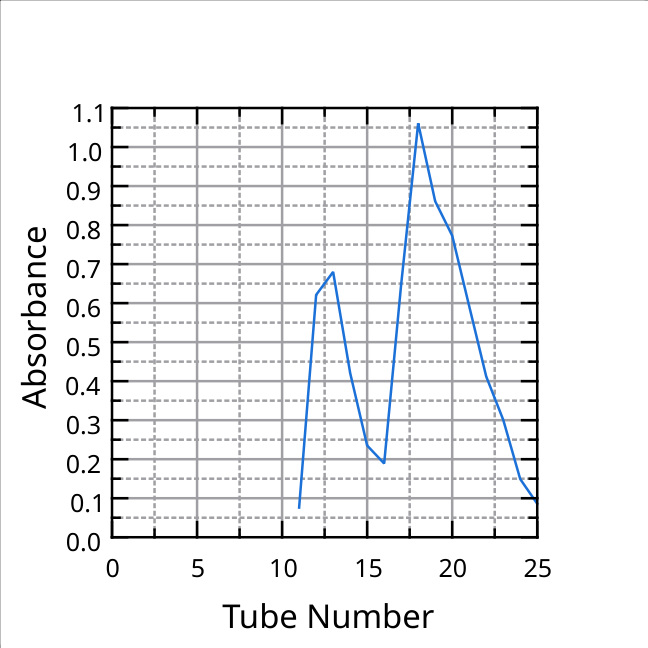
\includegraphics[width=0.45\textwidth]{bl.png}
\captionsetup{font={scriptsize,bf,stretch=1}}
\caption{\scriptsize \textbf{Absorbance Distribution of 25 tubes Containing Proteins b and c. Two peaks at positions 13 and 18 demonstrate that the bound proteins b and c after IEX are further separated from each other.}}
\label{fig3}
\end{figure}


\subsection{Spectrophotometry Scanning}
Measure the OD value of each tube to further confirm the tube with the highest concentration in the Bradford method. Additional scans are required to determine the optimal absorbance wavelength before actual measurement. Two absorption peaks were observed, with the absorbance at 548 nm being lower than that at 408 nm. Therefore 408 nm is more suitable as the measurement wavelength. It was confirmed that tubes 13 and 18 indeed had the highest protein concentrations required for the subsequent Bradford method, and that proteins b and c were successfully separated after GFC.


\subsection{Protein Concentration Calculation}
Using tubes 13 and 18, determine the concentration of relevant samples via Bradford in preparation for subsequent sample loading in SDS-PAGE and WB. The calibration results (Figure 3) show a high degree of fit. Properly dilute protein samples to ensure readings are within the range of the calibration curve. Results of the concentration calculations are presented in Table 3.


\begin{figure}[H]
\centering
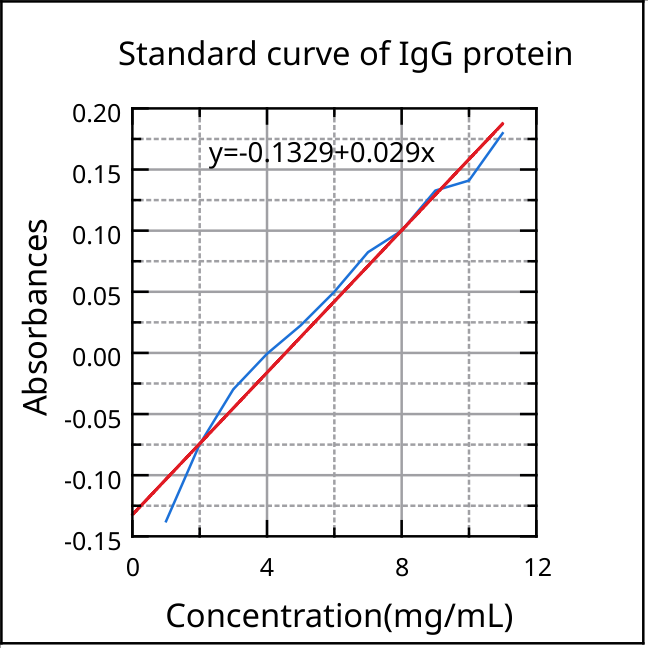
\includegraphics[width=0.45\textwidth]{igg.png}
\captionsetup{font={scriptsize,bf,stretch=1}}
\caption{\scriptsize \textbf{Calibrations of IgG concentration.}}
\label{fig4}
\end{figure}


\begin{center}
{Table 3. The Concentration of Protein Samples Through the Bradford Method.}
\vspace{0pt}
\begin{table}[H]
\setlength{\tabcolsep}{5pt}
\begin{tabular}{lc}
\toprule [1pt]
Components&Concentration(mg/mL)\\
\hline
Original Mixture & 5.2\\
IEX unbound & 1.7 \\
IEX bound & 4.3 \\
GFC peak 1 & 1.9 \\
GFC peak 2 & 2.0\\
\bottomrule [1pt]
\end{tabular}
\end{table}
\end{center}


\subsection{Bioinformatics Identification}
Bioinformatics analysis of proteins verified the applicability of the experimental method and prepared for the design of subsequent SDS-PAGE/WB experiments. The three distinct proteins—cytochrome c, myoglobin, and ferritin light chain—were inferred by BlastP searches of partial sequences. All partial sequences are 100\% identical. This illustrates the accuracy of protein identification. The MW and pI values are shown in Table 6 Myoglobin and cytochrome C as monomers have MWs of 11.83 kDa and 17.08 kDa, respectively, which is consistent with previous estimates in native gels. The MW of ferritin is 440 kDa, which is different from the predicted value. Therefore, the ferritin conformation observed in SDS-PAGE with a molecular weight of approximately 292 kDa may be a smaller oligomeric form or a degradation byproduct of the intact ferritin complex.

According to bioinformatics, to find a reasonable separation process, firstly cytochrome c is separated in IEX because its pI value is 9.59 and can pass through the anion exchange column. Sephacryl S-200 HR was used to separate the remaining two proteins. Because the MW of ferritin exceeds the 5-250 kDa separation range, ferritin is separated first in the GFC, followed by myoglobin.


\begin{center}
{Table 4. Data related to three proteins}
\vspace{0pt}
\begin{table}[H]
\setlength{\tabcolsep}{5pt}
\footnotesize
\begin{tabular}{llll}
\toprule [1pt]
Proteins&MW (kDa)& pI & Protein Fraction\\
\hline
Cytochrome c & 11.83 & 9.59 & IEX unbound\\
Myoglobin & 17.08 & 7.20 & GFC peak 2\\
Ferritin-light chain & 19.98 & 5.37 & GFC peak 1\\
Ferritin-heavy chain & 21.27 & 5.41 & GFC peak 1\\
\bottomrule [1pt]
\end{tabular}
\end{table}
\end{center}


\subsection{SDS-PAGE/WB Analysis}
SDS-PAGE/WB was further verified, and the results are shown in Figure 4 and Figure 5 respectively. The unbound IEX and GFC peaks 1/2 in SDS-PAGE have only one visible band per lane, indicating that the three proteins have been correctly separated by IEX and GFC with high protein purity and minimal protein degradation. The presence of two and three distinct bands in the IEX-bound and original mixtures indicates successful separation of cytochrome c in IEX. The positive control band indicates that the experiment was successful and can be applied to quantitative studies of proteins. In WB, anti-cytochrome c is used to localize and identify cytochrome c in the mixture. Bands were observed in the positive control, bound and unbound IEX groups. This parallels earlier protein isolation results and provides support for the physicochemical properties of cytochrome c and its involvement in the initial protein mixture.


The migration distance of a protein in SDS-PAGE is related to the MW of the protein, so it can be judged whether the MW of the protein analyzed by bioinformatics is consistent with the experimental value. Calculate the molecular weight of the protein to be tested by generating a standard curve using markers. The protein molecular weight determined by SDS-PAGE (Table 5) was found to be slightly higher than that found in the database, possibly due to protein conformation and gel modifications affecting migration rates. Two bright and dark bands near 26 kDa are visible in the lane containing ferritin. These bands represent the heavy and low chains of ferritin. Furthermore, wherever ferritin appears, there is a shallow band above 250 kDa, which may be due to insufficient denaturation and will require future work to characterize.


\begin{figure}[H]
\centering
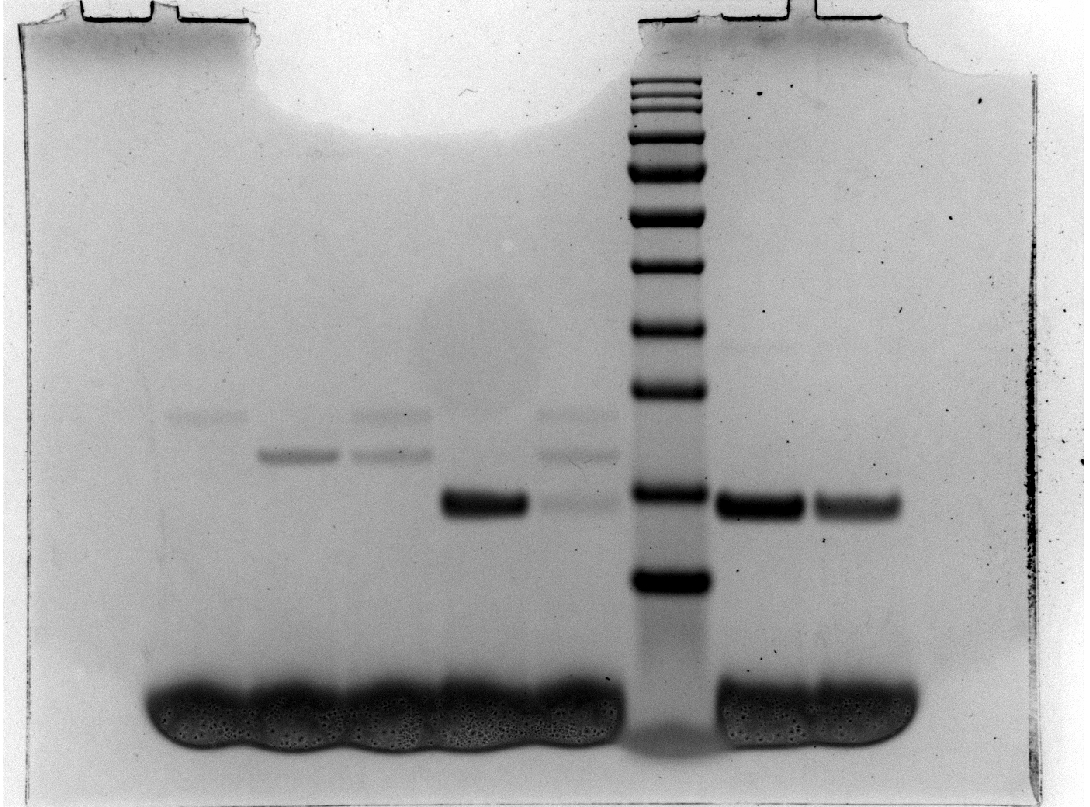
\includegraphics[width=0.45\textwidth]{G11.jpg}
\captionsetup{font={scriptsize,bf,stretch=1}}
\caption{\scriptsize \textbf{Results of Proteins Samples in 12\% gel of SDS-PAGE. The order of samples from left to right are tubes 12 and 20 in GFC purification, IEX bound, IEX unbound, Original mixture, and 0.25 and 0.125 mg/mL Cytochrome C.}}
\label{fig5}
\end{figure}


\begin{figure}[H]
\centering
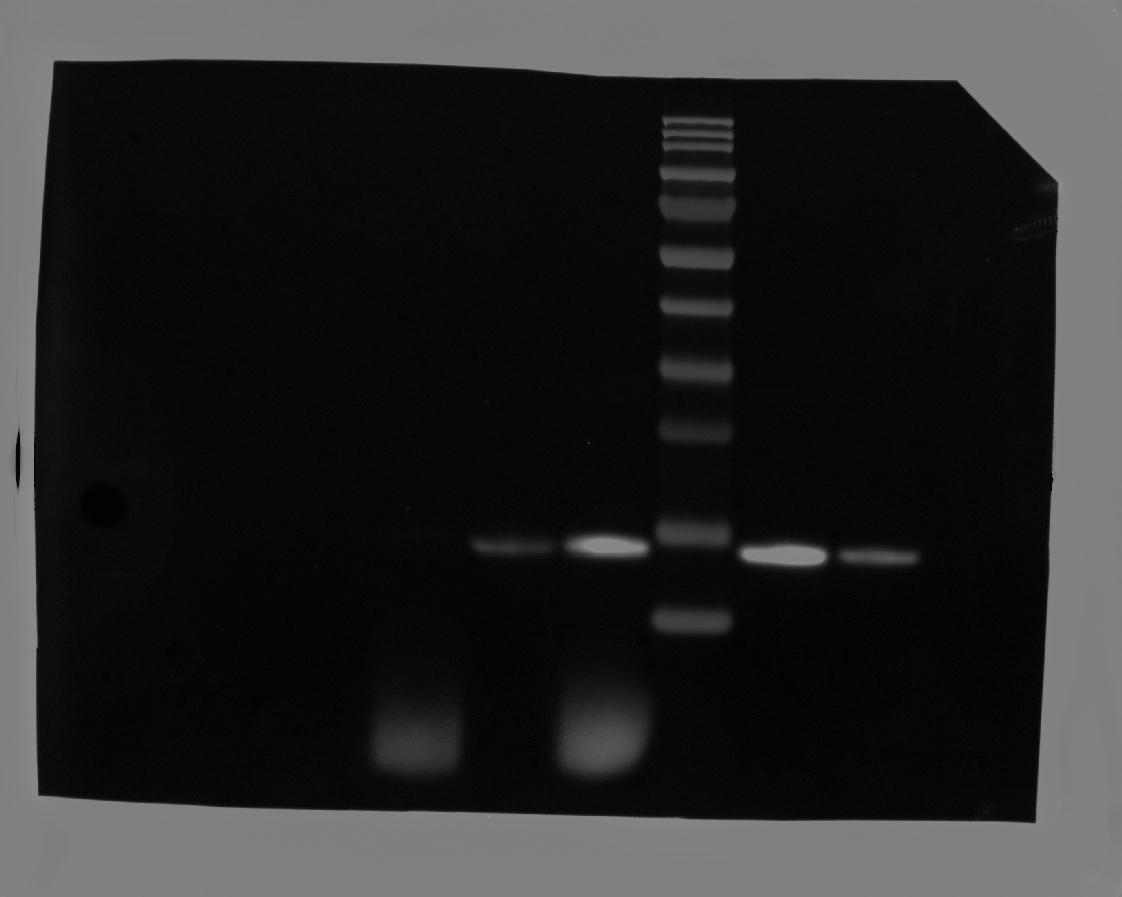
\includegraphics[width=0.45\textwidth]{G9(Composite).jpg}
\captionsetup{font={scriptsize,bf,stretch=1}}
\caption{\scriptsize \textbf{Results of Proteins Samples in WB. A goat anti-rabbit antibody conjugated to alkaline phosphatase served as the secondary antibody to the primary rabbit polyclonal antibody against Cytochrome c. The order of samples from left to right were tubes 12 and 20 in GFC purification, IEX bound, IEX unbound, original mixture, and 0.25 and 0.125 mg/mL Cytochrome C.}}
\label{fig6}
\end{figure}


\begin{center}
{Table 5. The Molecular Weight of Each Protein from SDS-PAGE and Bioinformatics Search.}
\vspace{0pt}
\begin{table}[H]
\setlength{\tabcolsep}{5pt}
\footnotesize
\begin{tabular}{llll}
\toprule [1pt]
Proteins&MW (database)&MW (SDS-PAGE)\\
\hline
Cytochrome c & 11.83 & 15.85\\
Myoglobin & 17.08 & 20.14\\
Ferritin-light chain & 19.98 & 23.61\\
Ferritin-heavy chain & 21.27 & 26.36\\
\bottomrule [1pt]
\end{tabular}
\end{table}
\end{center}


\section{Discussion and Conclusion}


The purpose of this experiment is to use different chromatographic methods to separate three unknown proteins, and then perform SDS-PAGE/WB and bioinformatics identification to further characterize the proteins. Two independent absorbance peaks after GFC and consistent band distribution by SDS-PAGE/WB demonstrate successful separation and reliable purity. Through a database search, three proteins were identified: cytochrome c, myoglobin, and ferritin. Most properties are consistent except for the molecular weight deviation of ferritin. The yields of cytochrome c, myoglobin, and ferritin calculated by the Bradford method were 1.7 mg/mL, 2.0 mg/mL, and 1.9 mg/mL, respectively. Theoretically, SDS-PAGE/WB results can also analyze protein concentration, but the grayscale of the bands will be inconsistent. Possible causes could include errors in the Bradford calibration or samples that were not completely mixed when loaded onto the gel, which could cause the protein content on the electrophoresis to actually be different.

There is a clear discrepancy between the predicted and actual molecular weights of ferritin, which may be explained by modifications to the gel and multi-subunit ferritin structures. As for the starting analysis, since native PAGE does not denature the structure of ferritin, molecular weight determination is likely to be strongly affected by interactions between subunits as well as overall protein conformation.

It is also worth noting that wherever ferritin is involved in SDS-PAGE, shallow bands appear that migrate much smaller distances or even lie outside the labeling range. Possible reasons may lie in incomplete denaturation or aggregation of ferritin. Although proteins are expected to be denatured and negatively charged when subjected to SDS-PAGE, ferritin is so large and complex that this process may not be ideal. These may result in slower migration that differs from the migration pattern of denatured heavy or light chains. Future work may use lower concentration polyacrylamide gels to ensure proper migration.


\bibliographystyle{unsrt}
\bibliography{reference}

\end{multicols}


\clearpage

\iffalse
\begin{appendices}
\section*{Appendix A. Data Analysis Sheet}\label{secA}

\textbf{Authors:} Mingbai.Zeng, Kangyao.Ma, Haozhan.Yuan, Yimeng.Yuan\\
\textbf{Date:} 2024.4.12\\
\textbf{Gene Name:} Uncharacterized\\
\textbf{Systemic Name:} AN8549, ANID\_08549\\
\textbf{Description:} Uncharacterized protein\\
\textbf{References:}For A. nidulans – none available\\
\textbf{GO annotation:}\\
GO:0008150 Biological Process\\
GO:0005575 Cellular Component\\
GO:0003674 Molecular Function\\
\textbf{S. cerevisiae Homologue:}\\
\textbf{Protein Sequence:}\\
\textgreater AN8549-T $\mid$ Aspergillus nidulans FGSC A4 $\mid$ segment length=394\\
\texttt{MPVDNYGVLKCRAITYKLEDGQQSPRAPQLSLYVRDTGSPTSQLNGHLQEARAGLPVHRAAINITSGDLDDSR\\
LAYWVNHQIGQNPIVNRLSQLEYGFHPVENNKTLGLDYIRDSLFTSTNGRLLPHDIPGQYTDIIDVLSPYIQH\\
AVREKANLYLFGSESRSDTRGSAPVIHNIHMNQGNARKFRADDGVFQDGGLIFHFPCARPDSDTGCVEDRPRG\\
EWLGIFLAFASQAVHTNPSSGHAISGVGWSDILRPDIIEEGVVIREARLHLDSSGTDADAVTDESETGARPCI\\
GRRKSISLTVTLSNHTNRAVRLGDWTIRNRSGCVHTLPRGIALRPMVDQHFELGDYTLSEDGDTILLLNEHGL\\
KVDGVSYNSAQEGMGLKGKGKGGSIVFVH}\\
\textbf{Pfam domains:}\\
1 Lamin tail domain superfamily, Lamin A/C globular tail domain\\
\textbf{Primers used for Deletion cassette:}\\
5 forward: \texttt{GTAACGCCAGGGTTTTCCCAGTCACGACGGAGACTCATACAGCCCTACC}\\
5 Reverse: \texttt{ATCCACTTAACGTTACTGAAATCTCAAGACCCCGTAGTTGTC}\\
3 forward: \texttt{CTCCTTCAATATCATCTTCTGTCGAGAGAAAAGGAGTGAGGTG}\\
3 Reverse: \texttt{GCGGATAACAATTTCACACAGGAAACAGCAAGCAGACAGTAACCCTAGC}\\
\textbf{Diagnostic primers and expected product size for wild type:}\\
ANID\_08549F: \texttt{TCGCAGGTCCCAGTGATG}\\
ANID\_08549R: \texttt{GTCCATCCCAGCCATTTG}\\
PCR product size in the wild type: 975 bp\\
\textbf{Diagnostic primers and expected product size for mutant:}\\
ANID\_08549F: \texttt{TCGCAGGTCCCAGTGATG}\\
Af-Rev: \texttt{CCACTTAACGTTACTGAAATC}\\
PCR product size in the mutant: 865 bp\\
\textbf{Annotated DNA sequence:}\\
(Note: The sequence in red indicates the intron of the genome, and the sequence in blue indicates the open reading frame (ORF) of the gene ANID\_08549 and PyrG gene. The sequences that are highlighted are the primers used in the lab session)
\begin{figure}[H]
\centering
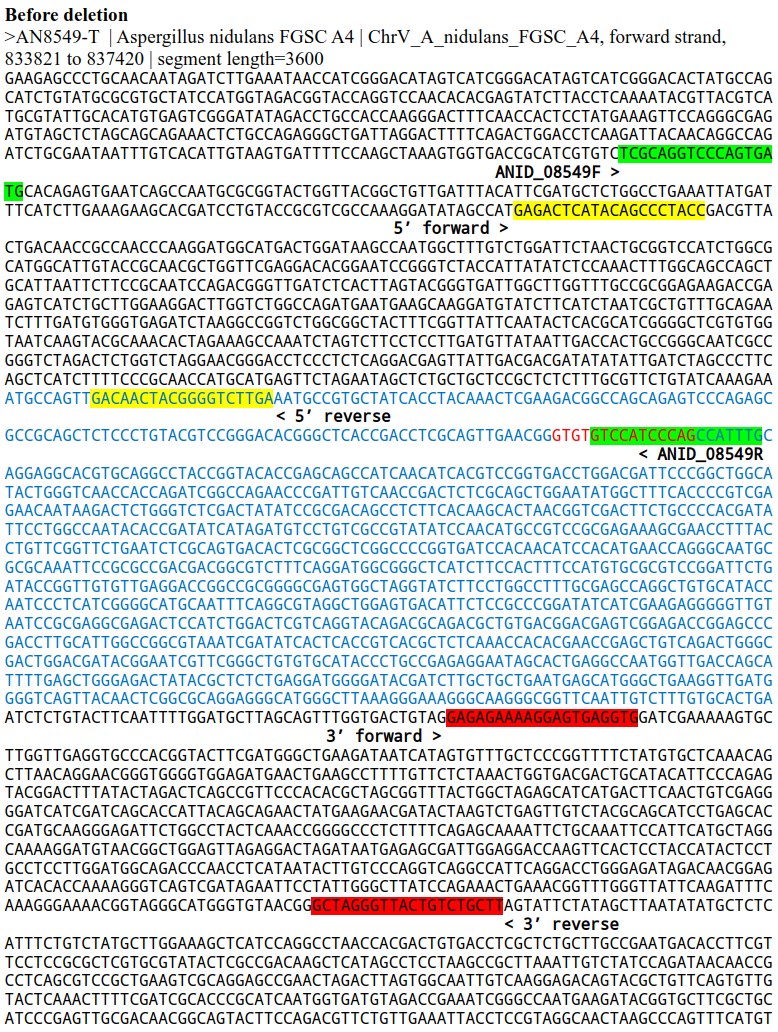
\includegraphics[width=0.95\textwidth]{before.png}
%\captionsetup{font={scriptsize,bf,stretch=1}}
%\caption{\scriptsize \textbf{Amplification of putative transformants and negative strain. Negative strain (A), transformants 1 (B) and transformant 2 (C).}}
%\label{fig4}
\end{figure}

\begin{figure}[H]
\centering
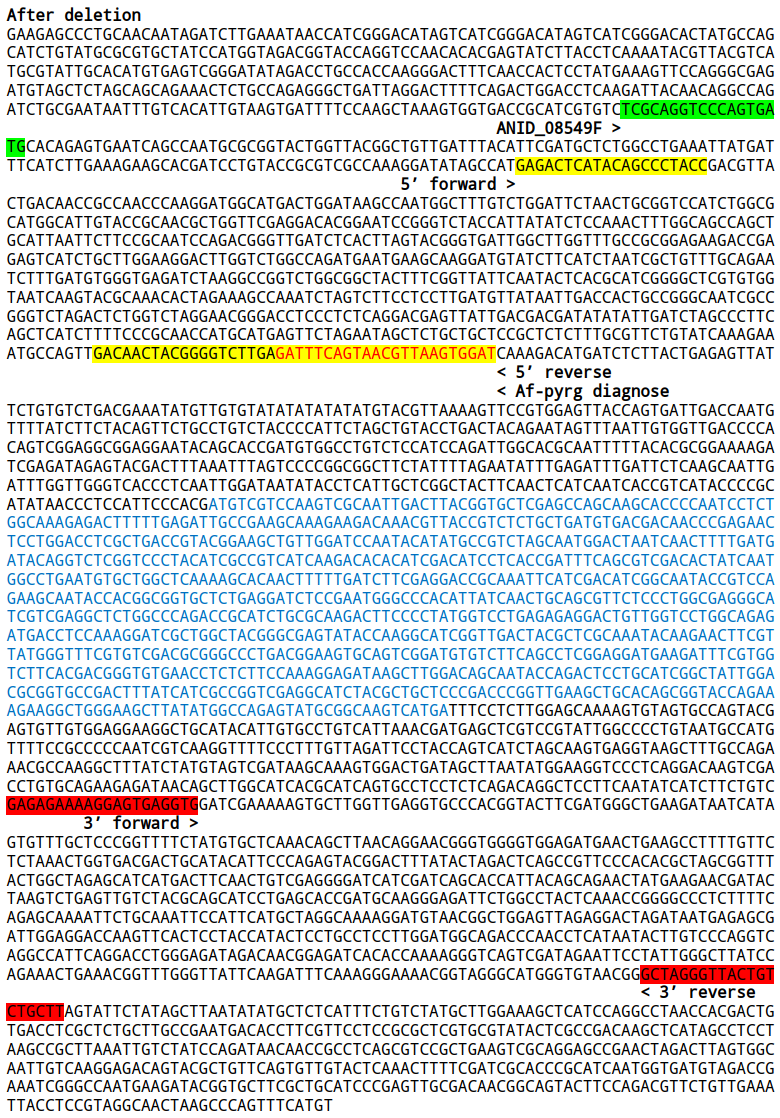
\includegraphics[width=0.95\textwidth]{after.png}
%\captionsetup{font={scriptsize,bf,stretch=1}}
%\caption{\scriptsize \textbf{Amplification of putative transformants and negative strain. Negative strain (A), transformants 1 (B) and transformant 2 (C).}}
%\label{fig4}
\end{figure}


\section*{Appendix B. Prediction of molecular structure of hypothetical protein AN8549}\label{secB}

\begin{figure}[H]
\centering
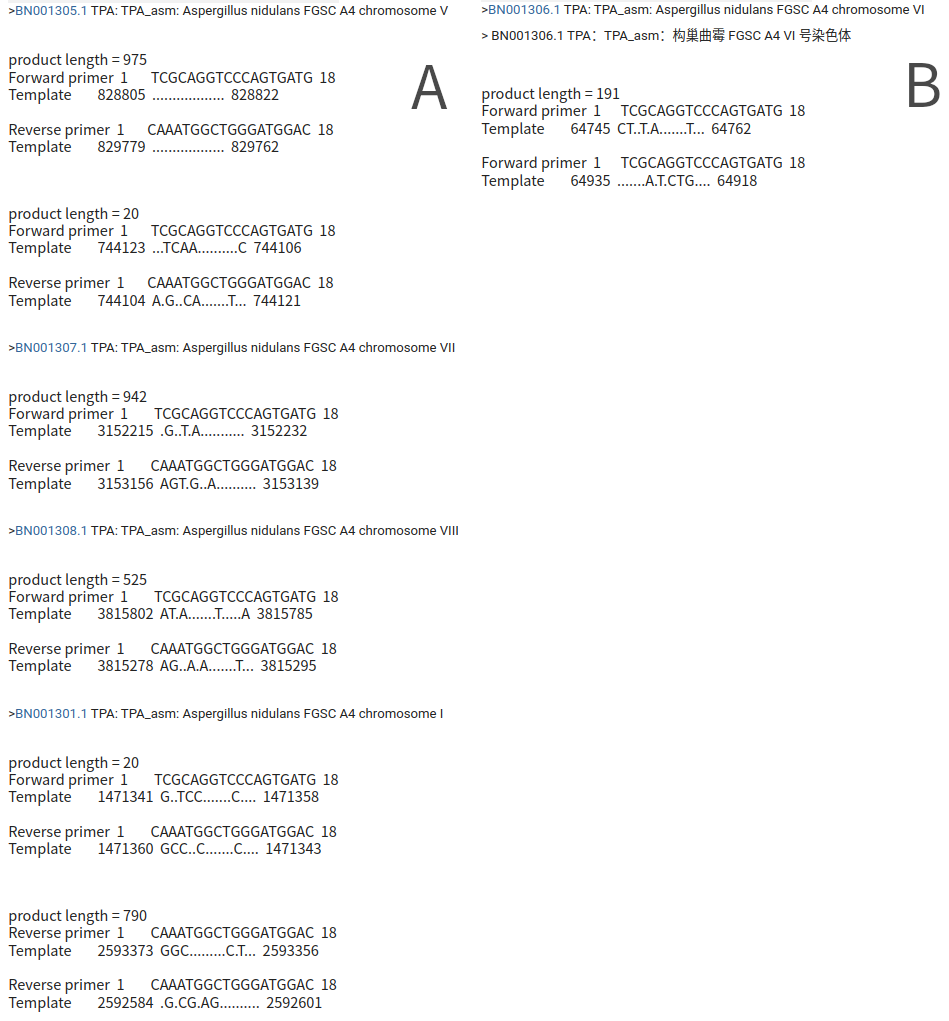
\includegraphics[width=0.95\textwidth]{primerblast.png}
%\captionsetup{font={scriptsize,bf,stretch=1}}
%\caption{\scriptsize \textbf{Amplification of putative transformants and negative strain. Negative strain (A), transformants 1 (B) and transformant 2 (C).}}
%\label{fig9}
\end{figure}


\section*{Appendix D. Prediction of domain structure of hypothetical protein AN8549\cite{paysan2023interpro}}\label{secD}

\begin{figure}[H]
\centering
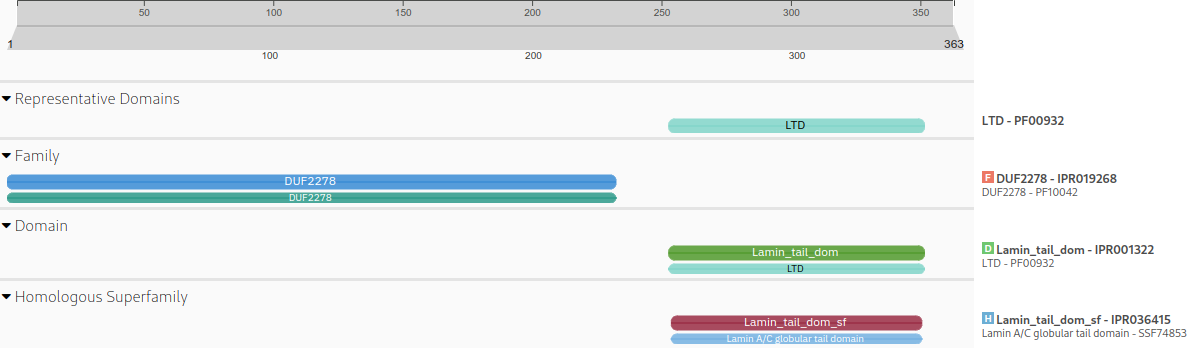
\includegraphics[width=0.95\textwidth]{BO83DRAFT_454721domain.png}
%\captionsetup{font={scriptsize,bf,stretch=1}}
%\caption{\scriptsize \textbf{Amplification of putative transformants and negative strain. Negative strain (A), transformants 1 (B) and transformant 2 (C).}}
%\label{fig5}
\end{figure}

\end{appendices}
\fi


\end{document}
